\chapter*{Part A\@:\\Deep Convolutional Neural Network}

\section*{Introduction}

The MNIST database of handwritten digits is a widely-used dataset to test image
recognition algorithms. It contains a training set of 60000 digits and a test
set of 10000 digits, each a centered image of size 28\(\times \)28.

Deep Convolutional Neural Network (DCNN) is a class of deep feedforward neural
networks that is considered a state-of-the-art approach in image recognition.
In this project, we would design a DCNN with an input layer, two convolutional
and maxpooling layers, a fully connected layer and an output softmax layer;
training and testing would be done on a subset of the MNIST dataset.

Three algorithms to update the weights are explored:
\begin{itemize}
    \item Stochastic Gradient Descent
    \item Stochastic Gradient Descent with Momentum
    \item RMSProp
\end{itemize}

\section*{Stochastic Gradient Descent (SGD)}

We have used up to 100 epochs; the following graph shows the training cost
against the number of epochs.

\begin{center}
    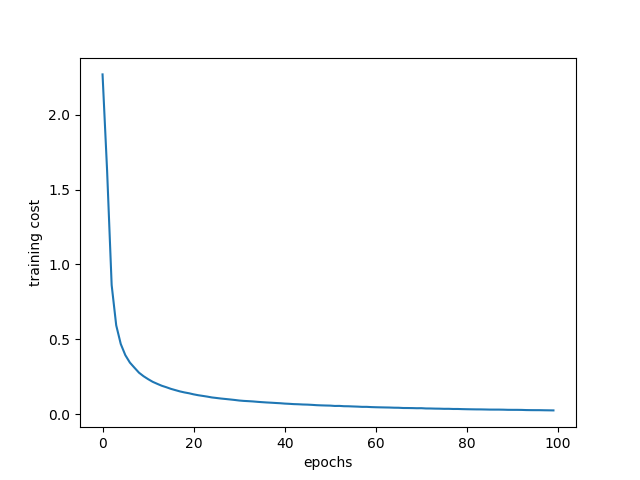
\includegraphics[width=\imgw]{project_2a_train_sgd}
\end{center}

The following graph shows the test accuracy against the number of epochs.

\begin{center}
    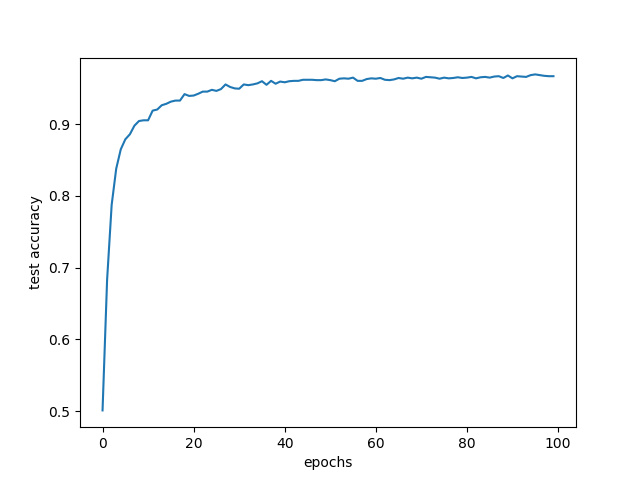
\includegraphics[width=\imgw]{project_2a_test_sgd}
\end{center}

Two images are chosen through setting different random seeds; the two seeds
are 10 and 42.

\begin{longtabu}{X[c]X[c]}
    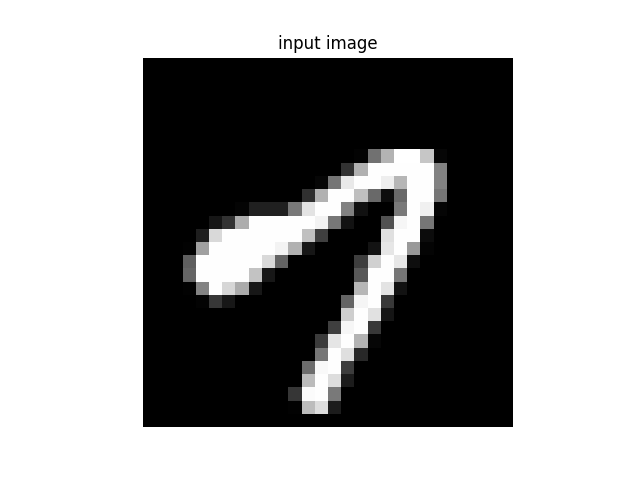
\includegraphics[width=\imgwt]{project_2a_sgd/img1_input} &
    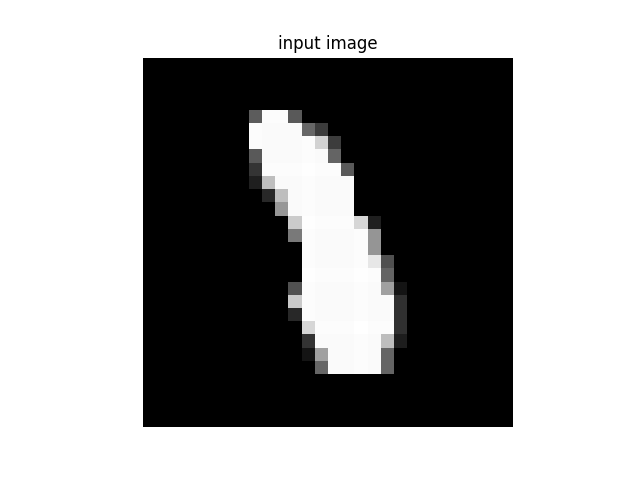
\includegraphics[width=\imgwt]{project_2a_sgd/img2_input}
\end{longtabu}

For image 1, the convolved and pooled feature maps are as follows:

\begin{longtabu}{X[c]X[c]}
    \includegraphics[width=\imgwt]{project_2a_sgd/img1_conv_1} &
    \includegraphics[width=\imgwt]{project_2a_sgd/img1_pooled_1} \\
    \includegraphics[width=\imgwt]{project_2a_sgd/img1_conv_2} &
    \includegraphics[width=\imgwt]{project_2a_sgd/img1_pooled_2}
\end{longtabu}

For image 2, the convolved and pooled feature maps are as follows:

\begin{longtabu}{X[c]X[c]}
    \includegraphics[width=\imgwt]{project_2a_sgd/img2_conv_1} &
    \includegraphics[width=\imgwt]{project_2a_sgd/img2_pooled_1} \\
    \includegraphics[width=\imgwt]{project_2a_sgd/img2_conv_2} &
    \includegraphics[width=\imgwt]{project_2a_sgd/img2_pooled_2}
\end{longtabu}

\section*{Stochastic Gradient Descent with Momentum}

The same 2 images are chosen.
For image 1, the convolved and pooled feature maps are as follows:

\begin{longtabu}{X[c]X[c]}
    \includegraphics[width=\imgwt]{project_2a_sgd_momentum/img1_conv_1} &
    \includegraphics[width=\imgwt]{project_2a_sgd_momentum/img1_pooled_1} \\
    \includegraphics[width=\imgwt]{project_2a_sgd_momentum/img1_conv_2} &
    \includegraphics[width=\imgwt]{project_2a_sgd_momentum/img1_pooled_2}
\end{longtabu}

For image 2, the convolved and pooled feature maps are as follows:

\begin{longtabu}{X[c]X[c]}
    \includegraphics[width=\imgwt]{project_2a_sgd_momentum/img2_conv_1} &
    \includegraphics[width=\imgwt]{project_2a_sgd_momentum/img2_pooled_1} \\
    \includegraphics[width=\imgwt]{project_2a_sgd_momentum/img2_conv_2} &
    \includegraphics[width=\imgwt]{project_2a_sgd_momentum/img2_pooled_2}
\end{longtabu}

\section*{RMSProp}

The same 2 images are chosen.
For image 1, the convolved and pooled feature maps are as follows:

\begin{longtabu}{X[c]X[c]}
    \includegraphics[width=\imgwt]{project_2a_rms_prop/img1_conv_1} &
    \includegraphics[width=\imgwt]{project_2a_rms_prop/img1_pooled_1} \\
    \includegraphics[width=\imgwt]{project_2a_rms_prop/img1_conv_2} &
    \includegraphics[width=\imgwt]{project_2a_rms_prop/img1_pooled_2}
\end{longtabu}

For image 2, the convolved and pooled feature maps are as follows:

\begin{longtabu}{X[c]X[c]}
    \includegraphics[width=\imgwt]{project_2a_rms_prop/img2_conv_1} &
    \includegraphics[width=\imgwt]{project_2a_rms_prop/img2_pooled_1} \\
    \includegraphics[width=\imgwt]{project_2a_rms_prop/img2_conv_2} &
    \includegraphics[width=\imgwt]{project_2a_rms_prop/img2_pooled_2}
\end{longtabu}

\section*{Analysis}

This graph shows the test accuracy against the number of epochs for
all three algorithms.

\begin{center}
    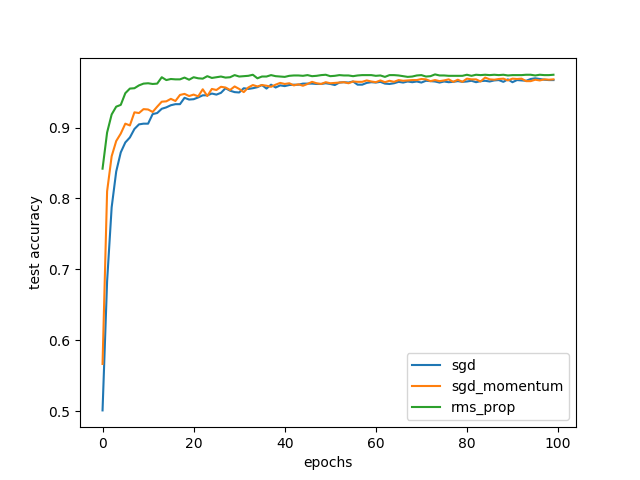
\includegraphics[width=\imgw]{project_2a_test}
\end{center}

The training time and training cost does not vary much between algorithms.
Different algorithms however extracts slightly different features from the
images, as evident from the feature maps, hence the difference in accuracy.
For the same random seed of 10, SGD achieves an accuracy of 97\%, SGD with
Momentum achieves 97.3\% and RMSProp achieves 98.0\%; this shows that
RMSProp gives the highest accuracy, and we could confidently conclude that
RMSProp is the best algorithm to use in this context.
